\documentclass[a4paper,11pt,fleqn]{article}
\usepackage{amsfonts}
\usepackage{amsthm}
\usepackage{graphicx}

\setlength{\parindent}{3em}
\setlength{\oddsidemargin}{0in}
\setlength{\textwidth}{6.5in} % sets 1in left and right margins
\setlength{\topmargin}{0.0in} % change to 0.2in for regular latex
%\setlength{\headheight}{0in}
%\setlength{\footheight}{0.5in}
\setlength{\footskip}{0.5in}
\setlength{\textheight}{9.0in} %sets 1in top and bottom margins
%\renewcommand{\baselinestretch}{1} %set to 1.5 for double spacing.


\newtheorem{Prop}{Proposition}
\newtheorem{lemma}{Lemma}

\newcommand{\br}{{\mathbf r}}
\newcommand{\bA}{{\mathbf A}}
\newcommand{\ba}{{\bf a}}
\newcommand{\bb}{{\bf b}}
\newcommand{\bc}{{\bf c}}
\newcommand{\bC}{{\bf C}}
\newcommand{\bd}{{\bf d}}
\newcommand{\be}{{\bf e}}
\newcommand{\bs}{{\bf s}}
\newcommand{\bn}{{\bf n}}
\newcommand{\bu}{{\bf u}}
\newcommand{\bv}{{\bf v}}
\newcommand{\bw}{{\bf w}}
\newcommand{\bx}{{\bf x}}
\newcommand{\by}{{\bf y}}
\newcommand{\bbf}{{\bf f}}
\newcommand{\bE}{{\bf E}}
\newcommand{\bL}{{\bf L}}
\newcommand{\bM}{{\bf M}}
\newcommand{\bN}{{\bf N}}
\newcommand{\bS}{{\bf S}}
\newcommand{\bT}{{\bf T}}
\newcommand{\bD}{{\bf D}}
\newcommand{\bX}{{\bf X}}
\newcommand{\bP}{{\bf P}}
\newcommand{\bI}{{\bf I}}
\newcommand{\bR}{{\bf R}}
\newcommand{\bU}{{\bf U}}
\newcommand{\bV}{{\bf V}}
\newcommand{\bW}{{\bf W}}
\newcommand{\bJ}{{\bf J}}
\newcommand{\bB}{{\bf B}}
\newcommand{\bzero}{{\bf 0}}
\newcommand{\bgamma}{{\mbox {\boldmath $\gamma$}}}
\newcommand{\btheta}{{\mbox {\boldmath $\theta$}}}
\newcommand{\bLambda}{{\mbox {\boldmath $\Lambda$}}}
\newcommand{\bPsi}{{\mbox {\boldmath $\Psi$}}}
\newcommand{\bPhi}{{\mbox {\boldmath $\Phi$}}}
\newcommand{\bcS}{{\mbox {\boldmath ${\cal S}$}}}
\newcommand{\bcH}{{\mbox {\boldmath ${\cal H}$}}}
\newcommand{\bcI}{{\mbox {\boldmath ${\cal I}$}}}
\newcommand{\bcR}{{\mbox {\boldmath ${\cal R}$}}}
\newcommand{\bcB}{{\mbox {\boldmath ${\cal B}$}}}

\title{ Semi-Blind Multiuser Detection }
\date{}
\author{LGE Mobile Research Center\\San Diego, CA 92131}
\begin{document}
\maketitle

\begin{abstract}

Multiuser detection is one of the key techniques for combating
multiple access interference (MAI) in CDMA systems. Most existing
semiblind/blind multiuser detectors are based the conventional
multiuser signal model or the subspace parametric model. In this
paper, we propose an different semiblind multiuser detection
framework based on a so-called semiblind signal model and
therefore two semiblind multiuser detectors using bestion linear
unbiased estimation (BLUE) and minimum mean squared error (MMSE)
estimation. Furthermore, the classic truncated-window scheme is
generalized to a multiple-window scheme which can detect several
consecutive bits at the same time. The proposed algorithms are
simple and direct. Only the desired user's timing, amplitude and
signature are required. No knowledge regarding other users is
involved. No search or convergence procedure is employed as in
many other semi-blind or blind detectors. Theoretical analysis and
computer simulations are also presented to support the performance
of the proposed semi-blind multiuser detection schemes.
\end{abstract}

\section{Introduction}

Direct-sequence code division multiple access (DS/CDMA) techniques
have attracted increasing attention for efficient use of available
bandwidth, resistance to interference and flexibility to variable
traffic patterns. One of the problems of such a system is the
so-called near-far problem resulting from excessive MAI energy
from nearby users compared with the desired user's signal energy.
Multiuser detection strategy is a method to minimize the effect of
MAI and solve the near-far problem in CDMA systems without a
significant reduction in the signal energies of the strong users
in order for the weaker users to achieve reliable communication.
It has been extensively investigated over the past several
years~\cite{Verd98}, since MAI is the dominant impairment for CDMA
systems and exists even in perfect power-controlled CDMA systems.

So far, most multiuser detection schemes are based on the
conventional multiuser signal model and then detect desired users
signal using the minimum bit-error rate, least-square errors,
minimum mean-squared error and/or minimum output energy criteria.  




Most early work on multiuser detection assumed that the receiver
knew the spreading codes or had some knowledge of all users, then
exploited this knowledge to combat MAI. For example, the classic
decorrelating detector for the synchronous case or the
single-truncated-window decorrelating detector for asynchronous
system can achieve the optimum near-far resistance and completely
eliminate MAI from other users with the expense of enhancement of
background noise. However, in many practical cases, especially in
a dynamic environment, e.g. in the downlink of a CDMA system, it
is very difficult for a mobile user to obtain accurate information
on other active users in the same channel. On the other hand, the
frequent use of training sequence is certainly a waste of channel
bandwidth. So blind multiuser detection has been proposed. Recent
research has been devoted to the blind multiuser receivers and
subspace-based signature waveform estimation schemes to achieve
better performance and higher capacity~\cite{Honi95, Poor97,
Wang98, Torl97, Liu96}. The minimum output energy (MOE) method and
subspace method were presented for multiuser blind detection with
the knowledge of only the desired users' spreading code and
possible timing.

An optimum near-far resistant multiuser detector which dose not
need power control has been proposed by Verd\'{u}~\cite{Verd89}.
However, its complexity is exponential in terms of the number of
users. That makes it unsuitable for practical situations. The
large gaps in performance and complexity between the conventional
single-user matched filter and optimum multiuser detector
encourage the search for other multiuser detectors that exhibit
good performance/complexity tradeoff. Suboptimum linear multiuser
detectors, which are based on linear transformation of the sampled
match filter outputs, were considered in~\cite{Lupa89} for
synchronous case. The decorrelating detector~\cite{Lupa89} not
only is a simple and nature strategy but also is optimal according
to three different criteria: least squares, near-far
resistance~\cite{Verd86} and maximum-likelihood when the received
amplitudes are unknown~\cite{Lupa89}. Though it does not require
knowledge of the received amplitudes, it does require the
information about other active users' signature waveforms. For the
asynchronous cases, Verd\'{u} suggested to use a one-shot version
of his decorrelating detector, the single-truncated-window
decorrelating detector, where one full-code matched filter is used
for the desired user and two partial-code matched filters are used
for each of the other users, where one of the two partial-code
mateched filter is matched to the {\em previous} part of its code
and the other one is matched to the {\em current} part of the
code. In this case, it not only requires the information about
other active users' signatures but also the time delay of other
users with respect to the desired user. Furthermore, since the
signature information of the other users is divided in a signature
matrix of the nearly doubled size, the performance of this
one-short single-truncated-window decorrelating detector is worse
than the complete asynchronous decorrelating detector.

It is shown in~\cite{Honi95} that the multiuser detector with
maximum output energy criteria is equivalent to that with the
linear minimum mean square error (MMSE) criteria. Compared the
optimal multiuser detection, they are near-far resistant and has
much less complexity. The major limitation of MOE schemes to
multiuser blind detection is that there is a saturation effect in
the steady state, which causes a significant performance gap
between the converged blind MOE and the true MMSE
detector~\cite{Honi95}.

Multiuser blind detection using subspace techniques was first
developed in depth by Wang and Poor~\cite{Wang98, Poor98}. Such
techniques were appropriate for the downlink environment where
only the desired user's code is available. More recently, these
subspace techniques were extended by Wang and
Host-Madsen~\cite{Wang99}, named group multiuser blind detectors,
to uplink environments where the base station knows the codes of
in-cell users, but not those of users outside the cell. In the
subspace-based blind detection approach~\cite{Wang98}, the linear
detectors are constructed in the closed form once the signal
subspace components are computed. That offers lower computational
complexity and better performance than the blind MOE detector. For
the subspace-based blind adaptive detector, the project
approximation subspace tracking deflation (PASTd)
algorithm~\cite{Yang95} is used to estimate the signal subspace.

As we see, various multiuser detection schemes have been developed
to combat the effects of MAI. These detection techniques either
assume the knowledge of all the users in the system (Conventional)
or assume the knowledge of the user of interest and without
knowledge of the channel input (Blind). Due to the limitation of
the blind algorithms in the presence of a large number of
interferers, there is a significant performance gap between these
two classes of detectors. In this work, we consider an
asynchronous DS/CDMA system and develop some partial blind
detectors, a new least squares semi-blind decorrelating detector
(LS-DD), a new total least squares semi-blind decorrelating
detector (TLS-DD) and a mixed LS/TLS semi-blind decorrelating
detector (MLS-DD). They are expected to bridge the performance gap
between the blind multiuser detectors and the conventional
multiuser detectors. In the proposed semi-blind multiuser
detectors, besides the desired user's timing and signature, the
amplitude is also required. So, we call them semi-blind detectors.
In the proposed algorithms, a new semi-blind signature matrix is
constructed with the desired user's signature and amplitude and
several previously received signal vectors. After this, the
decorrelating operation based on this new semi-blind signature is
proposed. With the analysis of the classic single-truncated-window
scheme, a new multi-window scheme is proposed to detect several
consecutive bits at the same time. That is expected to improve the
performance of the single-truncate-window algorithm. At last, the
LS, TLS and MLS version of the proposed semi-blind multi-window
decorrelating detection scheme are respectively proposed with
different assumptions regarding the noise in the proposed
semi-blind signature matrix. All these three algorithms are simple
and direct detection schemes. No knowledge of other users'
information is required. And no search or converging procedure is
employed as in many other semi-blind/blind detectors. Finally
theoretical analysis and computer simulations are also presented
to demonstrate the performance of the proposed semi-blind
decorrelating detectors.

The rest of the paper is organized as follows. In Section II, we
summarize the asynchronous signal model. In Section III, we review
the classic single-truncated-window decorrelating detector for
multiuser detection. In Section IV, the new data model with
multiple consecutive windows is discussed. In Section V, the
multi-window LS, TLS and MLS semi-blind decorrelating detection
algorithms are introduced. Performance analysis and simulation
results are provided in Section VI and VII. Section VIII concludes
this papers.

\section{Data Model and Problem Description}

A single-cell symbol-asynchronous DS/CDMA system over the
nondispersive additive white Gaussian noise (AWGN) channel is
considered. Spreading sequences are preassigned to all the active
users in the system and the signature waveform of the $k$th user
can be expressed as

\begin{equation}
\begin{array}{rcl}
s_k(t)&=&\sum\limits_{l=0}^{L-1}c_k^{(l)}\psi(t-lT_c)
\end{array}
\end{equation}

\noindent where $c_k^{(l)}\in \{-1/\sqrt{L},\ 1/\sqrt{L}\}$ is the
$l$th chip of the $k$th user's signature sequence, $L$ is the
spreading gain, $T_c$ is the chip interval and $\psi(t)$ is the
chip waveform. We assume that $\psi(t)$ satisfies the Nyquist
criterion for zero inter-chip interference and
$\int\limits_{-\infty}^{+\infty}|\psi(t)|^2dt=1$.

We consider reverse link transmission. The baseband representation
of the received signal due to the $k$th user is given by

\begin{equation}
\begin{array}{rcl}
r_k(t)&=&\sum\limits_{i=-\infty}^{+\infty}A_k b_k^{(i)}
s_k(t-iT_c-\tau_k)
\end{array}
\end{equation}

\noindent where $b_k^{(i)}$ is the $i$th bit sent by the $k$th
user. We assume that the $b_k^{(i)}$ is independent and
identically distributed random variables with $E\{b_k^{(i)}\}=0$
and $E\{|b_k^{(i)}|^2\}=1$. Also, $\tau_k$ denotes the
transmission delay from the $k$th user to the base station and
$A_k$ is the power of the received signal of the $k$th user. Then
the baseband signal at the input of the receiver at the base
station is

\begin{equation}
\begin{array}{rcl}
r(t)&=&\sum\limits_{k=1}^{K}r_k(t)+n(t)
\end{array}
\end{equation}

\noindent where $n(t)$ is additive white Gaussian noise with power
spectral density $\sigma_n^2$. We assume that there are $K$
simultaneous users in the system.

The received signal is synchronized for each user, passed through
the corresponding chip matched filter (CMF), and sampled at the
chip rate $1/T_c$. The vector of the output samples of the CMF for
$k$th user in the $n$th symbol interval can be expressed as

\begin{equation}
\begin{array}{rcl}
\br_k^{(n)}&=&\left[
\matrix{r_k(nT+T_c+\tau_k)&r_k(nT+2T_c+\tau_k)&\ldots&r_k(nT+LT_c+\tau_k)}\right]^T
\end{array}
\end{equation}

\noindent where

\begin{equation}
\begin{array}{rcl}
r_k(nT+lT_c+\tau_k)&=&\int\limits_{nT+lT_c+\tau_k}^{nT+(l+1)T_c+\tau_k}r_k(t)\psi(t)dt
\end{array}
\end{equation}

\noindent for $1\leq l \leq L$. To facilitate the analysis, we
will assume the system to be chip-synchronous and restrict
ourselves to the receiver that has an observation window of one
symbol interval. Without loss of generality. we consider the
detection of the first user. The observation window of the first
user is marked with a thick line in figure \ref{channel}. The
signals of other users are treated as interference. A typical
interferer has two different but consecutive symbols interfering
the symbol of user $1$, as shown in figure \ref{channel}. This can
be expressed as\footnote{Without loss of the generality, we will
drop the superscript $(n)$ from the vector $\br_1^{(n)}$ and
$\by_1^{(n)}$.}

\begin{figure}
\center{
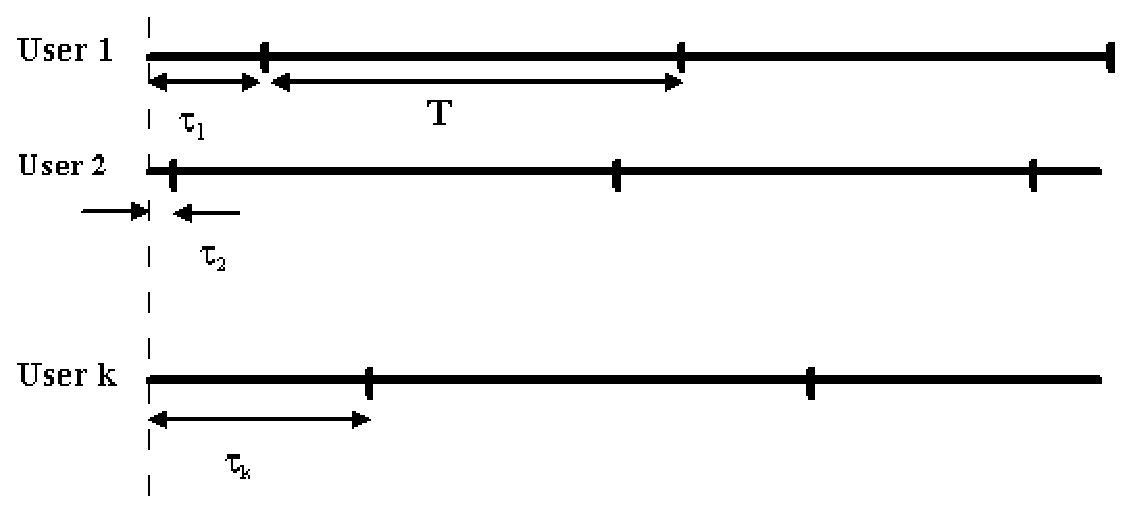
\includegraphics[width=6in]{AsynchCDMA.eps}}
\caption{The demonstration of a basic asynchronous multiuser
channel.}\label{channel}
\end{figure}

\begin{equation}
\begin{array}{rcl}
\br_1&=&A_1b_1^{(n)}\bs_1+\sum\limits_{k=2}^{K}A_k b_k^{(n-1)}
\bs_{k-}+\sum\limits_{k=2}^{K}A_k b_k^{(n)} \bs_{k+} + \bn
\end{array} \label{r}
\end{equation}

\noindent where $\bs_{k_-}$ and $\bs_{k_+}$ are named effective
signature sequences or part signature sequences that are
completely determined by the spreading sequences $\bs_k$ and the
delays relative to the first user $\tau_{k1}=\tau_k-\tau_1$, $\bn$
is an $L$-dimension Gaussian vector with independent
$\sigma_n^2$-variance components and $L \geq 2K-1$.

Now, the received signal vector $\br_1$ is fed into a correlating
receiver bank that is matched to each user's spreading waveform to
yield the output signal vector

\begin{equation}
\begin{array}{rcl}
\by_1&=&\bR(1)\bA\bb^{(n-1)}+\bR(0)\bA\bb^{(n)}+\bR^T(1)\bA\bb^{(n+1)}+\bar{\bn}
\end{array}
\end{equation}

\noindent where the zero-mean Gaussian process $\bar{\bn}$ has
autocovariance matrix

\begin{equation}
\begin{array}{rcl}
E\{\bar{\bn}_i\bar{\bn}_j^T\}&=&\left\{
\begin{array}{ll}
\sigma_n^2\bR^T(1)&j=i+1\\ \sigma_n^2\bR(0)&j=i\\
\sigma_n^2\bR(1)&j=i-1\\ \mathbf{0}&|j-i|>1
\end{array}\right.
\end{array}
\end{equation}

\noindent and the matrices $\bR(0)$ and $\bR(1)$ are defined by

\begin{equation}
\begin{array}{rcl}
R_{ij}(0)&=&\left\{
\begin{array}{ll}
1&j=i\\ \rho_{ij}&j<i\\ \rho_{ji}&j>i
\end{array}\right.
\end{array}
\end{equation}

\begin{equation}
\begin{array}{rcl}
R_{ij}(1)&=&\left\{
\begin{array}{ll}
0&j\geq i\\ \rho_{ij}&j<i
\end{array}\right.
\end{array}
\end{equation}

\noindent where, if $i\ge j$, then we denote

\begin{equation}
\begin{array}{rcl}
\rho_{ij}&=&\int\limits_{\tau}^{T}s_i(t)s_j(t-\tau)dt
\end{array},
\end{equation}

\begin{equation}
\begin{array}{rcl}
\rho_{ji}&=&\int\limits_{0}^{\tau}s_i(t)s_j(t+T-\tau)dt
\end{array}.
\end{equation}

Most of the linear multiuser detectors for demodulating the user's
data bit $b_1^{(n)}$ in (\ref{r}) is in the form of a correlator
followed by a hard limiter, which can be expressed as

\begin{equation}
\begin{array}{rcl}
\hat{b}_1^{(n)} &=& \mbox{sgn}\{\bw_1^T\br_1\}
\end{array} \label{linear}
\end{equation}

\noindent where $\bw_1 \in \mathbb{R}^{L\times 1}$.

Linear multiuser detectors can be implemented in a decentralized
fashion where only the user or users of interest need be
demodulated.

\section{Single-Truncated-Window Decorrelating Detector}

The large gaps in performance and complexity between the
conventional single-user matched filter and optimum multiuser
detector encourage the search for other multiuser detectors that
exhibit good performance/complexity tradeoffs. One of the earliest
suggestions to eliminate multiuser interference with a linear
receiver was proposed by Shnidman~\cite{Shni67}. The derivation of
the asymptotic efficiency of the decorrelating detector for
synchronous channels and the proof of its optimum near-far
resistant property are due to Verd\'{u}~\cite{Verd86} in the case
of nonsingular covariance matrices. The forerunner of the
decorrelating detector in the single-user intersymbol interference
(ISI) channel is the zero-forcing equalizer. And the counterpart
of decovariance in antenna array subject to undesired sources is
called null steering. Prior to developing the semi-blind
decorrelating detector, we discuss the classic
single-truncated-window decorrelating detector in the following,
which is useful in understanding the decorrelating detector.


As in equation (\ref{r}), the output vector of the receiver
outputs can be written as

\begin{equation}
\begin{array}{rcl}
\br_1&=&A_1b_1^{(n)}\bs_1+\sum\limits_{k=2}^{K}{A_k [
\matrix{\bs_{k-}&\bs_{k+}}] \left[\matrix{b_k^{(n-1)}\cr
b_k^{(n)}}\right]} + \bn\\

&=&\left[
\matrix{\bs_1&\bs_{2-}&\bs_{2+}&\ldots&\bs_{K-}&\bs_{K+}}\right]
\left[ \matrix{A_1&&&&&\cr &A_2&&&&\cr
&&A_2&&&\cr&&&\ddots&&\cr&&&&A_K&\cr&&&&&A_K}\right]
\left[\matrix{b_1^{(n)}\cr b_2^{(n-1)}\cr b_2^{(n)}\cr\vdots\cr
b_K^{(n-1)}\cr b_K^{(n)} }\right] + \bn\\ &=&\bS_1\bA_1\bb_1+\bn
\end{array}
\end{equation}

\noindent where

\begin{equation}
\begin{array}{rcl}
\bS_1&=&\left[\matrix{\bs_1&\bs_{2-}&\bs_{2+}&\ldots&\bs_{K-}&\bs_{K+}}\right]
\end{array}\hspace{0.1in},
\end{equation}

\begin{equation}
\begin{array}{rcl}
\bA_1&=&\mbox{diag}\left\{\matrix{A_1&A_2&A_2&\ldots&A_K&A_K}\right\}
\end{array}
\end{equation}

\noindent and

\begin{equation}
\begin{array}{rcl}
\bb_1&=&\left[\matrix{b_1^{(n)}&b_2^{(n-1)}&b_2^{(n)}&\ldots&b_K^{(n-1)}&b_K^{(n)}}\right]^T
\end{array}\hspace{0.1in}.
\end{equation}

\noindent The classic one-short decorrelating detector then
performs the following operation.

\begin{equation}
\begin{array}{rcl}
\hat{\bb}_1&=&\mbox{sgn}\{\bS_1^{+}\br_1\}
\end{array}
\end{equation}

\noindent where $[\star]^+$ denotes the Moore-Penrose generalized
inverse of $\star$.

In the classic single-truncated-window decorrelating detector, the
received vector $\br_1$ is projected on the subspace which is
orthogonal to the codes of the other users~\cite{Verd98,Tse99}.
Furthermore, in~\cite{Elda02}, it is shown that the above
decorrelating detector is the {\em oblique projection} of the
desired user's signature vector. That is to project $\bs_1$ onto
the orthogonal complement subspace of the space $\mathbb{S}_1$,
which is spanned by the other users' partial signature vectors,
along the null space of the space $\mathbb{S}_1$. The
decorrelating detector is designed to completely eliminate MAI
caused by other users, at the expense of enhancing the ambient
noise. So, the decorrelating detector is a sensible choice when
the received amplitudes are completely unknown. There are some
desirable features of this multiuser detector. It does not require
knowledge of the received amplitude, but it does require
$\bS_1^+$. It can readily be decentralized in the sense that the
demodulation of each user can be implemented completely
independently.


\section{New Data Model With Semi-Blind Signature Matrix}

Most of the multiuser detection schemes in the asynchronous case
assume the knowledge of the timing, the spreading codes and/or
channel parameters of all the users that contribute to the
received signal. Then these receivers would exploit this knowledge
to combat MAI. A second form of detectors, know as the blind
detectors, which operate without the knowledge of the channel
input and the information of other users. Usually, many practical
systems lie in between these two extremes. The first form of
detectors are too optimistic as we can not expect to know the
signature waveforms of all the users, while the latter
under-utilize the our knowledge of the system. In this section, we
will develop a new data model, where a new semi-blind signature
matrix with multiple consecutive windows is proposed. Based this
data model, the semi-blind decorrelating detectors can be proposed
in the next section and they are expected to bridge the
performance gap between the conventional detectors and blind ones.

It is widely known that the performance of the
single-truncated-window decorrelating detector is worse than that
of the asynchronous decorrelator in terms of both bit-error rate
(BER) and near-far resistance (NFR)~\cite{Verd98}. This is because
that, in the classic one-shot single-truncated-window
decorrelating detector, the energy of each interfering signal is
separated in a signature matrix of the larger columns, $2K-1$, so
that the single-truncated-window crosscovariance matrix may be
more easily singular, even when the corresponding $K\times K$
asynchronous crosscovariance matrix is not singular. Hence, we
propose to use multiple consecutive windows instead of the single
window in this section. We will see that, except the first and
last window, there is no broken interferering signal vector or
signature any more. This is expected to improve the performance of
decorrelating detectors for asynchronous systems.

Without loss of the generality, we only detect the information
signal bits sent by user $1$ at $P$ consecutive symbol intervals
$t\in [(n-P+1)T_s,\ nT_s]$, where $P$ is the length of the
consecutive truncated windows. The $P$ consecutive information
bits for user $1$ in the signal vector $\bb_1$ can be detected
simultaneously. To this end, the new $PL\times M$ semi-blind
signature matrix $\bcS$ for user $1$ is defined as

\begin{equation}
\begin{array}{rcl}
\bcS&=&[\matrix{\bar{\bs}_1&\bar{\bs}_2&\bar{\bs}_3&\ldots&\bar{\bs}_M}]\\
 &=&[\matrix{\bI_P \otimes (A_1\bs_1)&\bar{\br}_{1}&\bar{\br}_{2}&\ldots&\bar{\br}_{M-P}}]\\
 &=&\left[\matrix{\bS\bA\bE&\bS\bA\bar{\bb}_1&\bS\bA\bar{\bb}_2&\ldots&\bS\bA\bar{\bb}_{M-P}}\right]+ \bar{\bN}\\
 &=&\bS\bA\left[\matrix{\bE&\bar{\bb}_1&\bar{\bb}_2&\ldots&\bar{\bb}_{M-P}}\right]+ \bar{\bN}\\
 &=&\bS\bA\left[\matrix{\bE & \bD }\right]+ \bar{\bN}\\
 &=&\bS\bA\bB + \bar{\bN}
\end{array} \label{S}
\end{equation}

\noindent where the $PL\times (PK+K-1)$ matrix
$\bS=[\matrix{\bar{\bS}_1&\bar{\bS}_2&\bar{\bS}_3&\ldots&\bar{\bS}_K}]$
is the multi-window signature matrix, in which

\begin{equation}
\begin{array}{rcccl}
\bar{\bS}_1&=&\bI_P\otimes\bs_1
&=&\mbox{diag}\{\matrix{\bs_1&\bs_1&\ldots&\bs_1}\}_{PL\times P}
\end{array}
\end{equation}

\noindent and

\begin{equation}
\begin{array}{rcl}
\bar{\bS}_k&=&\mbox{diag}\{\matrix{\bs_{k_-}&\bs_k&\ldots&\bs_k&\bs_{k_+}}\}_{PL\times
(P+1)}
\end{array},
\end{equation}

\noindent the $(PK+K-1)\times (PK+K-1)$ diagonal matrix
$\bA=\mbox{diag}\{\matrix{\bar{\bA}_1&\bar{\bA}_2&\ldots&\bar{\bA}_K}\}$
\noindent denotes the multi-window signal amplitude matrix, in
which

\begin{equation}
\begin{array}{rcl}
\bar{\bA}_1&=&\mbox{diag}\{\matrix{A_1&A_1&\ldots&A_1}\}_{P\times
P}
\end{array}
\end{equation}

\noindent and

\begin{equation}
\begin{array}{rcl}
\bar{\bA}_k&=&\mbox{diag}\{\matrix{A_k&A_k&\ldots&A_k}\}_{(P+1)\times
(P+1)}
\end{array},
\end{equation}

\noindent $\bar{\br}_i$ are the arbitrary received vectors,
$\otimes$ denotes the Kronecker product,
$\bE=\left[\matrix{\bI_P&\mathbf{0}}\right]^T$, the $(PK+K-1)
\times 1$ vector $\bar{\bb}_i$ is one of the multi-window bit
vectors consisting of bits previously sent by the $K-1$
interfering users, the $PL\times(M-P)$ matrix $\bD = [\bar{\bD}^T\
\tilde{\bD}^T]^T$ denotes the multi-window information bit matrix,
in which the $(M-P)\times P$ vector $\bar{\bD}$ is the information
vector consisting of the known bits previously sent by the desired
user and $\mbox{rank}\{\tilde{\bD}\}=PK+K-P-1$, the $PL\times M$
matrix $\bar{\bN}=[\mathbf{0}\ \tilde{\bN}]$ denotes the
multi-window noise matrix,
\begin{equation}
\begin{array}{rcl}
 \bB&=&\left[\matrix{\bE &\bD }\right]\\
 &=&\left[\matrix{\bC \cr \matrix{\mathbf{0}& \tilde{\bD}}
 }\right]\\
 &=&\left[\matrix{\bI_P& \bar{\bD} \cr \mathbf{0}& \tilde{\bD} }\right]

\end{array}
\end{equation}

\noindent and $\mbox{rank}\{\bB\}=PK+K-1$, $i=1,\ 2,\ \ldots,\
M-P$, $k=2,\ 3,\ \ldots,\ K$. We maintain  $PL\geq M\geq PK+K-1$.

With equation (\ref{r}) and (\ref{S}), the relationship between
the current received signal vector $\br$, which consists of $P$
consecutively received signal vectors by the desired user, and the
new semi-blind signature matrix $\bcS$ can be expressed as

\begin{equation}
\begin{array}{rcl}
\br&=&[\matrix{\br_1^{(n)T}&\br_1^{(n-1)T}&\ldots&\br_1^{(n-P+1)T}}]^T\\
 &=&\bS\bA\bb + \bn\\
 &=&\bS\bA\bB\bB^{+}\bb + \bn\\
 &=&(\bcS-\bar{\bN})\bB^{+}\bb + \bn\\
 &=&\bcS\bB^{+}\bb-\bar{\bN}\bB^{+}\bb + \bn\\
 &=&\bcS\bd + \tilde{\bn} \label{rn}
\end{array}
\end{equation}

\noindent where

\begin{equation}
\begin{array}{rcl}
\bb&=&\left[\matrix{\bar{\bb}^T&\tilde{\bb}^T}\right]^T\\
&=&\left[\matrix{\left[\matrix{b_1^{(n)}\cr
b_1^{(n-1)}\cr\vdots\cr
b_1^{(n-P+1)}}\right]^T&\left[\matrix{b_2^{(n)}\cr b_2^{(n-1)}\cr
\vdots\cr b_2^{(n-P+1)}\cr
b_2^{(n-P)}}\right]^T&\cdots&\left[\matrix{b_K^{(n)}\cr
b_K^{(n-1)}\cr \vdots\cr b_K^{(n-P+1)} \cr
b_K^{(n-P)}}\right]^T}\right]^T,
\end{array}
\end{equation}


\noindent in which the $P\times 1$ vector
$\bar{\bb}=\left[\matrix{b_1^{(n)}&b_1^{(n-1)}&\cdots&b_1^{(n-P+1)}}\right]^T$
denotes the desired bit vector of user $1$, the $M \times 1$
vector $\bd$ denotes the new detection vector and is defined as

\begin{equation}
\begin{array}{rcl}
\bd&=&\bB^+\bb\\
 &=&\left[\matrix{\bE&\bD}\right]^+\bb\\
 &=&\left[\matrix{\bI_P&\bar{\bD}\cr\mathbf{0}&\tilde{\bD}}\right]^+\left[\matrix{\bar{\bb}\cr\tilde{\bb}}\right]
\end{array} \label{DetectorVector}
\end{equation}

\noindent and $\tilde{\bn}$ is the new noise vector and defined as

\begin{equation}
\begin{array}{rcl}
\tilde{\bn}&=&\bn-\bar{\bN}\bB^{+}\bb
\end{array} \label{new_noise}
\end{equation}

\noindent With the following lemma, it is easy to see that the new
semi-blind noise item $\tilde{\bn}$ is enhanced, compared with the
former noise item $\bn$. This enhancement is because there is the
noise matrix $\bar{\bN}$ existing in the semi-blind signature
matrix $\bcS$.


Now, the following result can be easily proved.
\begin{Prop}
The Moor-Penrose general inverse of $\bB$ is
\begin{equation}
\begin{array}{rcl}
\bB^{+}&=&\left[\matrix{\bE&\matrix{\bar{\bD}\tilde{\bD}^{+}\cr\tilde{\bD}^{+}}}\right]
\end{array}
\end{equation}\label{Prop_B}
\end{Prop}

\begin{proof}

Based on the definition of $\bB$,

\begin{equation}
\begin{array}{rcl}
\bB&=&\left[\bE\ \matrix{\bar{\bD}\cr\tilde{\bD}}\right]
\end{array}
\end{equation}

\noindent so that

\begin{equation}
\left[\bE\ \matrix{\bar{\bD}\cr\tilde{\bD}}\right]\left[\bE\
\matrix{\bar{\bD}\tilde{\bD}^{+}\cr\tilde{\bD}^{+}}\right]
=\left[\matrix{\bI_P&\bar{\bD}\cr\mathbf{0}&\tilde{\bD}}\right]\left[\matrix{\bI_P&-\bar{\bD}\tilde{\bD}^{+}\cr\mathbf{0}&\tilde{\bD}^{+}}\right]
=\bI_{PK+K-1}
\end{equation}
where $\bI_{PK+K-1}$ is the unitary matrix of the size
$(PK+K-1)\times (PK+K-1)$.
\end{proof}

With Proposition \ref{Prop_B}, the detection vector $\bd$ can be
re-written as

\begin{equation}
\begin{array}{rcl}
\bd&=&\left[\matrix{\bar{\bd}\cr\tilde{\bd}}\right]\\
 &=&\left[\matrix{\bE&\matrix{\bar{\bD}\cr\tilde{\bD}}}\right]^{+}\left[\matrix{\bar{\bb}\cr\tilde{\bb}}\right]\\
 &=&\left[\matrix{\bI_P&-\bar{\bD}\tilde{\bD}^{+}\cr\mathbf{0}&\tilde{\bD}^{+}}\right]\left[\matrix{\bar{\bb}\cr\tilde{\bb}}\right]\\
 &=&\left[\matrix{\bar{\bb}-\bar{\bD}\tilde{\bD}^{+}\tilde{\bb}\cr\tilde{\bD}^{+}\tilde{\bb}}\right]
\end{array}
\end{equation}

\noindent where the $P\times 1$ matrix $\bar{\bd}$ denotes the
first consecutive $P$ elements of the detection vector $\bd$ as

\begin{equation}
\bar{\bd}=\bar{\bb}-\bar{\bD}\tilde{\bD}^{+}\tilde{\bb}
\end{equation}

\noindent and $\tilde{\bd}$ is the complement vector as

\begin{equation}
\tilde{\bd}=\tilde{\bD}^{+}\tilde{\bb}
\end{equation}


Now, the following result can be very easily reached.

\begin{lemma}
The bits vector $\bar{\bb}$ which consists of the bits sent by
user 1 at $P$ consecutive time intervals $t=n-P+1$, $n-P+2$,
$\ldots$, $n$ can be got with the following equation.
\begin{equation}
\begin{array}{rcl}
\bar{\bb}&=& \bC\bd\\
 &=& [\matrix{\bI_P&\bar{\bD}}]\bd\\
 &=&\bar{\bd}+\bar{\bD}\tilde{\bd}
\end{array}
\end{equation} \label{bn_estimation}
\end{lemma}

We can see that, after the definition of the new semi-blind
signature matrix $\bcS$ in equation (\ref{S}), the form of the
classic multiuser detection model can still be kept as in equation
(\ref{rn}). But the different is that, the information bit vector
$\bb$ is replaced by the detection vector $\bd$ as in equation
(\ref{DetectorVector}) and the original AWGN noise vector $\bn$ is
replace by the new noise vector $\tilde{\bn}$ as in equation
(\ref{new_noise}). Fortunately, with lemma \ref{bn_estimation}, it
still is possible for us to calculate the desired bit vector
$\bar{\bb}$ with the detection vector $\bd$ and the previously
detected bits matrix $\bC$. The next question then is how to
estimate the detection vector $\bd$ as efficiently as possible. In
the following section, there are three estimation schemes proposed
for the estimation of $\bd$. They are LS, TLS and MLS estimation
schemes.

On the other hand, as we may see, the classic
single-truncated-window scheme for the asynchronous case can be
taken as a special case of the presented multi-window scheme with
$P=1$. In the single-truncated-window scheme, there is no complete
signature of other user existing in the signature matrix. This
makes its inverse unstable. But, in the presented multi-window
scheme, there are $P-1$ complete signature vectors of any other
user in the new constructed signature matrix. Hence, the inverse
of the multi-window signature matrix should be much more stable
than that of the single-truncated-window signature matrix.

\section{One-Shot Multi-Windows Semi-Blind Decorrelating Detection}

In the previous section, the principles of the proposed semi-blind
decorrelating detection scheme are described. With lemma
\ref{bn_estimation}, the detection of the desired information bit
vector $\bar{\bb}$ can be decided by the estimation of the
detection vector $\bd$. The left problem is how to estimate the
vector $\bd$. In this section, we are going to propose three
algorithms to estimate $\bd$ with the difference assumptions
regarding the noise matrix $\bar{\bN}$ in the semi-blind signature
matrix $\bcS$. Also, following the different estimation schemes of
the detection vector $\bd$, three different multi-window
semi-blind detectors are proposed.

\subsection{Least-Square Semi-Blind Decorrelating Detector}

At first, the measurements of $\bcS$ is assumed to be free of
error and all errors are confined to the received vector $\br$ as
in equation (\ref{rn}). The following least-square estimation of
the detection vector $\bd$ is then proposed.

\begin{lemma}~\cite{Golu96} Suppose $\bU^T\bcS\bV=\mathbf{\Sigma}$ is the SVD of $\bcS\in\mathbb{R}^{PL\times
 M}$ with $r=rank(\bcS)$. And if $\bU=[\matrix{\bu_1&\bu_2&\ldots&\bu_{PL}}]$,
 $\bV=[\matrix{\bv_1&\bv_2&\ldots&\bv_M}]$, $\mathbf{\Sigma}=diag\{[\matrix{\sigma_1&\ldots\sigma_r&0&\ldots&0}]\}$ and $\br\in\mathbb{R}^{PL\times 1}$, then

 \begin{equation}
 \matrix{\bd_{LS}=\sum\limits_{i=1}^{r}\frac{\bu_i^T\br}{\sigma_i}\bv_i=\bcS^+\br}
 \end{equation}

\noindent minimizes $\|\bcS\bd-\br\|_2$ and has the smallest
2-norm of all minimizers. Moreover
 \begin{equation}
 \matrix{\varepsilon_{LS}^2 = \min\limits_{\bx\in\mathbb{R}}\|\bcS\bx-\br\|_2^2 &=& \sum\limits_{i=r+1}^{L}(\bu_i^T\br)^2}
 \end{equation}
\label{VectorLS}
\end{lemma}

\begin{proof}
For any $\bx\in\mathbb{R}^{K\times 1}$, we have

\begin{equation}
\begin{array}{rcl}
\|\bcS\bx-\br\|_2^2&=&\|(\bU^T\bcS\bV)(\bV^T\bx)-\bU^T\br\|_2^2\\
        &=&\|\mathbf{\Sigma}\mathbf{\alpha}-\bU^T\br\|_2^2\\
        &=&\sum\limits_{i=1}^{r}(\sigma_i\alpha_i-\bu_i^T\br)+\sum\limits_{i=r+1}^{m}(\bu_i^T\br)^2
\end{array}
\end{equation}

\noindent where $\mathbf{\alpha} = \bV^T\bx$. Clearly, if $\bx$
solves the least-square problem, then $\alpha_i =
\bu_i^T\br/\sigma_i$ for $i=1,\ 2,\ \ldots,\ r$. If we set
$\alpha_{r+1}=\alpha_{r+2}=\ldots=\alpha_{M}$, then the resulting
$\bx=\bd_{LS}$ clearly has minimal 2-norm.
\end{proof}

So, the least-square estimation of $\bd$ is

\begin{equation}
\begin{array}{rcl}
\bd_{LS} &=& \bcS^+\br\\
 &=&\bd + \bcS^+\tilde{\bn}
\end{array} \label{LS}
\end{equation}

\noindent And, the linear filter bank representation $\bW_{LS}$ in
the proposed LS semi-blind decorrelating detector is

\begin{equation}
\begin{array}{rcl}
\bW_{LS}&=&(\bC\bcS^+)^T
\end{array} \label{w_LS}
\end{equation}

And, the block of bits $\bar{\bb}$ sent by the first user during
the time interval $t\in[(n-P)T,\ nT]$ can be detected with the
following equation.

\begin{equation}
\begin{array}{rcl}
\bar{\bb}_{LS}&=&\mbox{sgn}\{\bW_{LS}^{T}\br\}\\
&=&\mbox{sgn}\{\bC\bd_{LS}\}\\
 &=&\mbox{sgn}\{[\matrix{\bI_P&\bar{\bD}}](\bd + \bcS^+\tilde{\bn})\}\\
 &=&\mbox{sgn}\{\bar{\bb}+[\matrix{\bI_P&\bar{\bD}}]\bcS^+\tilde{\bn}\}
\end{array} \label{b_LS}
\end{equation}

\subsection{Total Least-Square Semi-Blind Decorrelating Detector}

It is easy to find that the above least-square estimation of
detection matrix $\bd$ is the minimum norm solution to the
following equation,

\begin{equation}
\begin{array}{rcl}
\matrix{\min\limits_{\bx}\left\|\br-\bcS\bx\right\|_2}&\mbox{subject
to}&\br\subseteq \mathbb{R}(\bcS)
\end{array}.\label{LSProb}
\end{equation}

\noindent It is assumed that the semi-blind signature matrix
$\bcS$ is error-free. However, this assumption is not true with
its definition as in the equation (\ref{S}). Obviously, there is
the noise item $\bar{\bN}$ exiting.

On the other hand, $\br$ can also be expressed as

\begin{equation}
\begin{array}{rcl}
\br&=&\bS\bA\bb + \bn\\
 &=&\bS\bA\bB\bB^{+}\bb + \bn\\
 &=&(\bcS-\bar{\bN})\bB^{+}\bb + \bn\\
 &=&\hat{\bcS}\bd + \bn
\end{array}
\end{equation}

\noindent where  $\hat{\bcS}=\bcS-\bar{\bN}=\bS\bA\bB$. Hence, the
estimation of $\bd$ can easily be transformed into the following
total least-square problem

\begin{equation}
\begin{array}{rcl}
\matrix{\min\limits_{\bar{\bcS},\ \bx}\left\|\left
[\matrix{\bcS&\br}\right]-\left[\matrix{\bar{\bcS}&\bar{\bcS}\bx}\right]\right\|_2}
&\mbox{subject to}&\br\subseteq\mathbb{R}(\bar{\bcS})
\end{array}\hspace{0.1in}.
\label{TLSProb}
\end{equation}

\begin{lemma}\cite{Huff91} Let $\bcS=\bU^{'}\mathbf{\Sigma}^{'}\bV^{'T}$ and
$[\matrix{\bcS&\br}]=\bU\mathbf{\Sigma}\bV^T$ be the SVD of $\bcS$
and $[\matrix{\bcS&\br}]$, respectively. If $\sigma_{M}^{'}
> \sigma_{M+1}$, then

\begin{equation}
\begin{array}{rcl}
\bd_{TLS}&=&(\bcS^T\bcS-\sigma_{M+1}^2\bI)^{-1}\bcS^T\br
\end{array}
\end{equation}
and
\begin{equation}
\begin{array}{rcccl}
\varepsilon_{TLS}^{2}&=&\min\limits_{\bx\in \mathbb{R}^{M\times
1}}\|\bcS\bx-\br\|_2^2&=&\sigma_{M+1}^2\left[1+\sum\limits_{i+1}^{M}{(\bu_i^{'T}\br)^2
\over \sigma_i^{'2}-\sigma_{M+1}^2 }\right]
\end{array}
\end{equation}
\noindent where

\noindent $\bU=[\matrix{\bu_1&\bu_2&\ldots&\bu_{PL}}]$,
$\bV=[\matrix{\bv_1&\bv_2&\ldots&\bv_{M+1}}]$,
$\mathbf{\Sigma}=\mbox{diag}\{[\matrix{\sigma_1&\ldots&\sigma_{M+\min\limits\{PL-M,\
1\}}}]\}$ \noindent and
$\bU^{'}=[\matrix{\bu_1^{'}&\bu_2^{'}&\ldots&\bu_{PL}^{'}}]$,
 $\bV^{'}=[\matrix{\bv_1^{'}&\bv_2^{'}&\ldots&\bv_{M}^{'}}]$,
 $\mathbf{\Sigma}^{'}=\mbox{diag}\{[\matrix{\sigma_1^{'}&\sigma_2^{'}&\ldots\sigma_M^{'}}]\}$;
\end{lemma}


So, the total least-square estimation of $\bd$ is

\begin{equation}
\begin{array}{rcl}
\bd_{TLS}&=&(\bcS^T\bcS-\sigma_{M+1}^2\bI)^{-1}\bcS^T\br
\end{array}
\end{equation}

The linear filter representation of the presented total
least-squaer semi-blind decorrelating detector is

\begin{equation}
\begin{array}{rcl}
\bW_{TLS}&=&\bC^T(\bcS^T\bcS-\sigma_{M+1}^2\bI)^{-1}\bcS^T
\end{array}
\end{equation}

And, the block of  bits $\bar\bb$ sent by the first user during
the time interval $t\in[(n-P)T,\ nT]$ can be detected with the
following equation,

\begin{equation}
\begin{array}{rcl}
\bar{\bb}_{TLS}&=&\mbox{sgn}\{\bW_{TLS}^T\br\}\\
 &=&\mbox{sgn}\{\bC^T\bd_{TLS}\}\\
 &=&\mbox{sgn}\{[\matrix{\bI_P&\bar{\bD}}](\bcS^T\bcS-\sigma_{M+1}^2\bI)^{-1}\bcS^T\br\}
% &=&\mbox{sgn}\{b_n^1+[\matrix{A_1^{-1}&\bar{\bd}^T}]\bcS^+\tilde{\bn}\}
\end{array} \label{b_TLS}
\end{equation}

\subsection{Mixed LS/TLS Semi-Blind Decorrelating Detector}

In the least-square estimation of $\bd$, it assumes that the
signature matrix $\bcS$ is noise-free. In total least-square
estimation of $\bd$, it assumes that there is noise in each
element of $\bcS$. However, we can see that, except the first $P$
columns of $\bcS$ are exactly known to be noise/error-free, there
are noise existing in each element of its rest $M-P$ columns. To
maximize the accuracy of the estimated detection vector $\bd$, it
is natural to seek the best fitting solution that is appropriate
to the received signal vector $\br$ and the polluted $M-P$ columns
in the semi-blind signature matrix $\bcS$, while keeping the
exactly known $P$ columns of $\bcS$ unperturbed. Thus, the problem
to estimate the detection vector $\bd$ can easily be transformed
into the following mixed LS/TLS estimation problem.

\begin{equation}
\begin{array}{rcl}
\matrix{\min\limits_{\hat{\bar{\bcS}},\
\bx}\left\|\left[\matrix{\bar{\bcS}&\br}\right]-\left[\matrix{\hat{\bar{\bcS}}&[\matrix{\bar{\bS}_1\bar{\bA}_1&\hat{\bar{\bcS}}}]\bx}\right]\right\|_{2}
}&\mbox{subject
to}&\br\subseteq\mathbb{R}([\matrix{\bar{\bS}_1\bar{\bA}_1&\hat{\bar{\bcS}}}])
\end{array}\label{MLSProb}
\end{equation}

This mixed LS/TLS problem can be solved with the following lemma.

\begin{lemma}~\cite{Huff91} Consider the mixed least squares and total least squares problem in equation (\ref{MLSProb}) and perform the householder transformations $Q$ on the matrix
$[\matrix{\bcS&\br}]$ so that

\begin{equation}
\begin{array}{rcl}
Q^H[\matrix{\bar{\bS}_1\bar{\bA}_1&\bar{\bcS}&\br}]&=&\left[\matrix{\bR_{11}&\bR_{12}&\bR_{1r}\cr
\mathbf{0}&\bR_{22}&\bR_{2r}}\right]
\end{array}
\end{equation}

\noindent where $\bR_{11}$ is a $P\times P$ upper triangle matrix,
$\bR_{12}$ is a $P\times (M-P)$ matrix, $\bR_{22}$ is a
$(L-P)\times (M-P)$ matrix , $\bR_{1r}$ is a $P\times 1$ vector
and $\bR_{2r}$ is a $(L-P)\times 1$ vector.

Denote $\sigma'$ the smallest singular value of $\bR_{22}$ and
$\sigma$ the smallest singular value of
$[\matrix{\bR_{22}&\bR_{2r}}]$. If $\sigma'>\sigma$, then the MLS
solution uniquely exists and is given by

\begin{equation}
\begin{array}{rcl}
\bd_{MLS}&=&\left(\bcS^T\bcS-\sigma^2\left[\matrix{\mathbf{0}&\mathbf{0}\cr\mathbf{0}&\mathbf{I}_{M-P}}\right]\right)^{-1}\bcS^T\br
\end{array}.
\end{equation}
\end{lemma}

So, the linear filter representation of the presented MLS
semi-blind decorrelating detector is

\begin{equation}
\begin{array}{rcl}
\bW_{MLS}&=&\bcS\left(\bcS^T\bcS-\sigma^2\left[\matrix{\mathbf{0}&\mathbf{0}\cr\mathbf{0}&\mathbf{I}_{M-P}}\right]\right)^{-1}\bC^T
\end{array}
\end{equation}

And, the block of bits $\bar\bb$ sent by the first user during the
time interval $t\in[(n-P)T\ nT]$ can be detected with the
following equation.

\begin{equation}
\begin{array}{rcl}
{\bar\bb}_{MLS}&=&\mbox{sgn}\{\bW_{MLS}^{T}\br\}\\
 &=&\mbox{sgn}\left\{[\matrix{\bI_P&\bar{\bD}}]\left(\bcS^T\bcS-\sigma^2\left[\matrix{\mathbf{0}&\mathbf{0}\cr\mathbf{0}&\mathbf{I}_{M-P}}\right]\right)^{-1}\bcS^T\br\right\}\\
 &=&\mbox{sgn}\{\bC\bd_{MLS}\}\\
 &=&\mbox{sgn}\{[\matrix{\bI_P&\bar{\bD}}]\bd_{MLS}\}\hspace{0.1in}.
\end{array}\label{b_MLS}
\end{equation}


\section{Performance Analysis}

\subsection{The Relationship Between the Semi-Blind Signature Matrix $\bcS$ and the Signature Matrix $\bS$}

As we may see, one of the most different between the classic
single-truncated-window decorrelating detector and the proposed
semi-blind decorrelating detector is the definition of the
signature matrix. When $P=1$, the proposed semi-blind signature
matrix $\bcS$ is composed with the desired user's signature and
$M-1$ uncorrelated previously received vector as the rest columns
while the original signature matrix $\bS$ is defined with the
desired user's complete signature vector and all the other users'
partial signature vectors. When $\bar{\bN} = \mathbf{0}$, it is
very easy to see that these two signal subspaces,
$\mbox{span}\{\bS\}$ and $\mbox{span}\{\bcS\}$, are the same one.

\subsection{The Relationship Between Decorrelating Detector and LS Semi-Blind Detector }

When there is no noise the semi-blind signature matrix $\bcS$,
$\hat{\bcS}=\bcS$ and $\tilde{\bn}=\bn$. When
$\bar{\bN}=\mathbf{0}$ and $P=1$, there is the following
relationship between the first user's LS semi-blind decorrelating
detector $\bw_{LS}$ and its classic single-truncated-window
decorrelating detector $\bw_{DD}$.

\begin{equation}
\begin{array}{rcl}
\bw_{LS}&=&A_1^{-1}\bw_{DD}
\end{array}
\end{equation} \label{wN0}

\noindent Furthermore, the classic decorrelating detector can be
taken as a special case of the semi-blind decorrelating detector
with $\bB =\bI$. And the output of the limiter of the LS
semi-blind decorrelating detector is

\begin{equation}
\begin{array}{rcl}
b_{LS}&=&\mbox{sgn}\{b_1+A_1^{-1}\bS^+\bn\}
\end{array} \label{b_LS_N0}
\end{equation}

At this time, the bit-error-rate of the user 1 with the presented
LS semi-blind decorrelating detector is same to that with
single-truncated-window decorrelating detector. It can be
expressed as

\begin{equation}
\begin{array}{rcl}
P_{e}&=&Q\left({A_1\over \sigma_{n}\sqrt{R_{11}^+}}\right)
\end{array}
\end{equation}

\noindent where $R_{11}^+$ is a shorthand for $(\bR^{-1})_{11}$,
the $1$th row and $1$th column element in the matrix
$\bR^{-1}=(\bS^T\bS)^{-1}$.

Thus, the presented LS semi-blind detector at this time achieves
the maximum near-far resistance as the classic
single-truncated-window decorrelating detector does.

\subsection{The Relationship Between $\bar\bb$ and $\bd$}

We can see that the detection vector $\bd$ plays the key pole in
the proposed semi-blind decorrelating detectors. When there is no
estimation error in the detection vector $\bd$, with Lemma
\ref{bn_estimation}, the desired bit vector $\bar\bb$ could
exactly be estimated from the detection vector $\bd$ and $\bC$.
When the detection vector $\bd$ cannot be exactly estimated, the
relationship between the estimation errors of $\bar\bb$ and $\bd$
is

\begin{equation}
\begin{array}{rcl}
\Delta b_p&\leq&\|\Delta\tilde{\bd}\|_1+|\bar{d}_p|
\end{array}\label{b_error}
\end{equation}

\noindent where $b_p$ denotes the $p$th element of vector $\bb$,
$\hat{b}_p$ is a estimate of $b_p$, $\Delta b_p=\hat{b}_p-b_p$,
$\Delta\tilde{\bd}=\hat{\tilde{\bd}}-\tilde{\bd}$, $\bar{d}_p$
denotes the $p$th element of $\bar\bd$ and $\|\star\|_1$ denotes
the 1-norm of the vector $\star$.

\subsection{The Relationship between the Noise Items $\tilde{\bn}$ and $\bn$}

With the following lemma, it is easy to see that the new
semi-blind noise item $\tilde{\bn}$ is enhanced compared to the
former noise item $\bn$. This enhancement is because there is the
noise $\bar{\bN}$ existing in the semi-blind signature matrix
$\bcS$.

The mean of the semi-blind noise item $\tilde{\bn}$ which is
defined in equation (\ref{new_noise}) is

\begin{equation}
\begin{array}{rcccl}
\tilde{m}&=&E\{\tilde{\bn}\}&=&0
\end{array}
\end{equation}

The variance of the semi-blind noise item $\tilde{\bn}$ satisfies
the following inequation

\begin{equation}
\begin{array}{rcccl}
\max\{var\{\tilde{\bn}\}\}&=&\max\{E\{(\tilde{\bn}-\tilde{m})^2\}\}&\leq&\sigma_n^2+(P+1)(K-1)\|\tilde{\bD}^+\|_2^2\sigma_{\bar{n}}^2
\end{array} \label{noise_mean}
\end{equation}
\noindent where $\max\{\star\}$ denotes the maximum item in the
vector $\star$ and $\sigma_{\bar{n}}^2$ is the power of the noise
item $\bar{\bN}$ in the semi-blind signature matrix $\bcS$.

\section{Computer Simulations}

In this section, various computer simulations and analytical
results are presented. In the computer simulations, two users are
sending the signals in asynchronous CDMA system. The spreading
gain $g=24$. the covariance matrix between these two users are
$\bR$.

\begin{equation}
\begin{array}{rcl}
\bR&=&\left[\matrix{\bs_1^T\cr\bs_{2_-}^{T}\cr\bs_{2_+}^{T}}\right][\matrix{\bs_1&\bs_{2_-}&\bs_{2_+}}]\\
    &=&\left[\matrix{1.0000&-0.6250&-0.0417\cr
                    -0.6250& 0.8750&      0\cr
                    -0.0417&      0& 0.1250}\right]
\end{array}
\end{equation}

\noindent and the channel is AWGN channel. We do the simulations
with $P=1$, $2$, $3$, $4$, $5$, $7$ and $9$. Correspondingly, the
number of columns in the semi-blind signature matrix is
$M=(P+1)\times K-1$. We will compare our algorithms with
single-user matched filter (MF) detector and the
single-truncated-window decorrelating detector (DD).

\subsection*{case 1: $\bar{\bN} = \mathbf{0}$}

In this case, we suppose that there is no noise in the semi-blind
signature matrix $\bcS$ or the noise is negligible, compared to
the noise in the received signal vectors. With the theoretical
analysis before, since there is no noise or the noise is
negligible in the semi-blind signature matrix, only the LS
semi-blind detector is examined and compared to the single-user
matched filter detector and the single-truncated-window
decorrelating detector in this case.

\begin{figure}
\center{
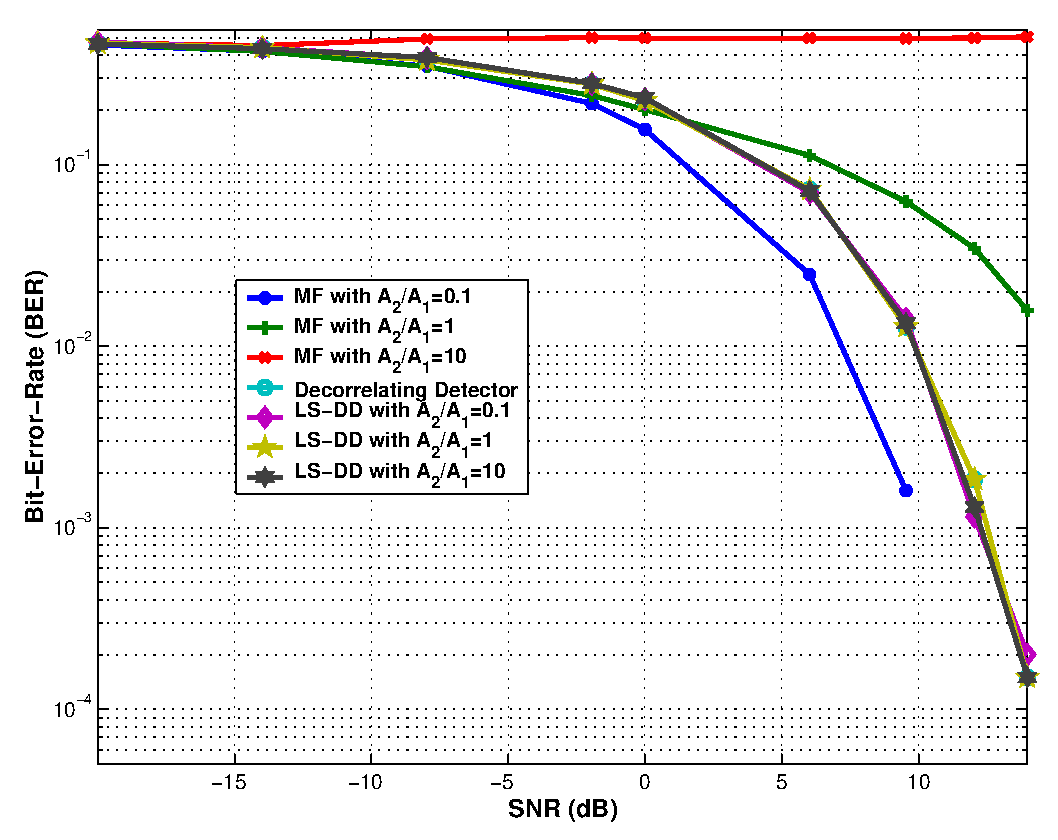
\includegraphics[width=4in]{BER_LS10.eps}}
\caption{Bit-error-rate comparison of the signal-user matched
filter, decorrelating detector, and the presented LS semi-blind
detector with $P=1$ for the first user within two users.}
\label{LS10}
\end{figure}

\begin{figure}
\center{
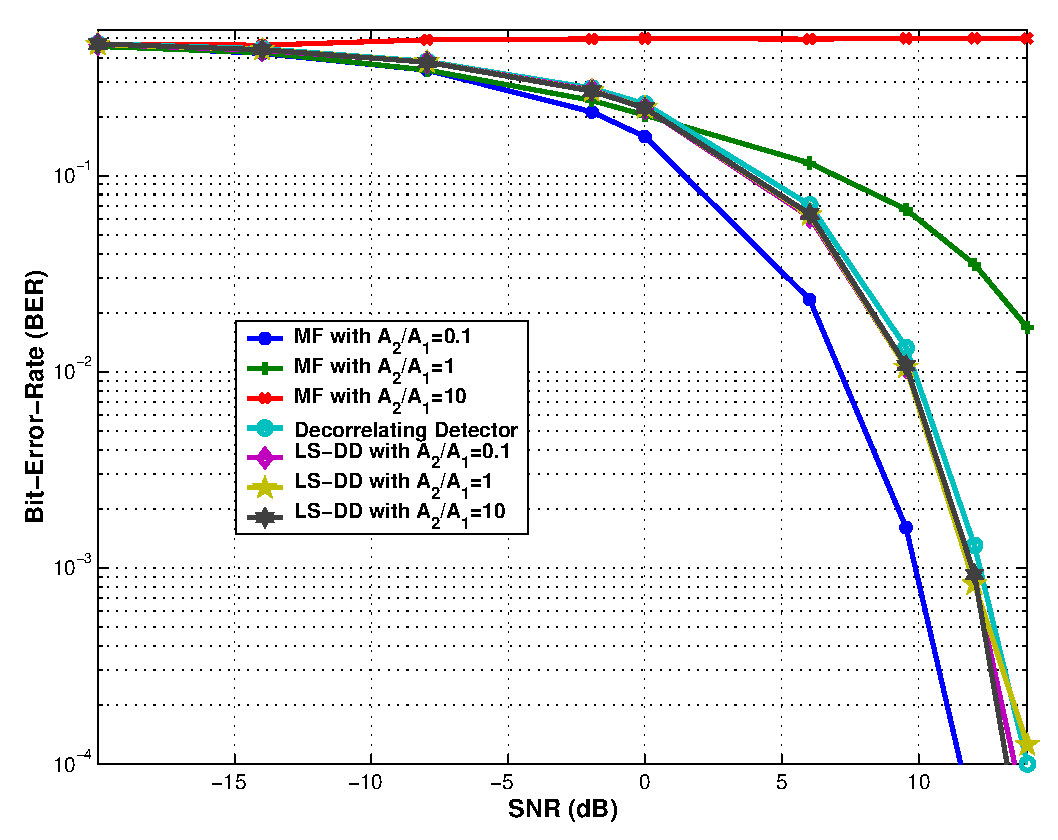
\includegraphics[width=4in]{BER_LS40.eps}}
\caption{Bit-error-rate comparison of the signal-user matched
filter, decorrelating detector, and the presented LS semi-blind
detector with $P=4$ for the first user within two users.}
\label{LS40}
\end{figure}

As we see in figure \ref{LS10}, the performance of the LS
semi-blind detector with $P=1$ is very close to that of the
single-truncated window decorrelating detector. This also supports
that the classic single-truncated-window decorrelating detector
just is a special case of the proposed LS-DD detector with
$\bar{\bN} = \mathbf{0}$ and $\bB=\bI$. Comparing figure
\ref{LS40} to figure \ref{LS10}, the performance of the LS-DD with
four consecutive windows ($P=4$) is a little bit better than that
of the LS-DD with single truncated window ($P=1$) and the classic
single-truncated-window decorrelating detector. As we analyzed
before, it is because that more complete signatures of other users
are employed in th semi-blind signature matrix $\bcS$.

\begin{figure}
\center{
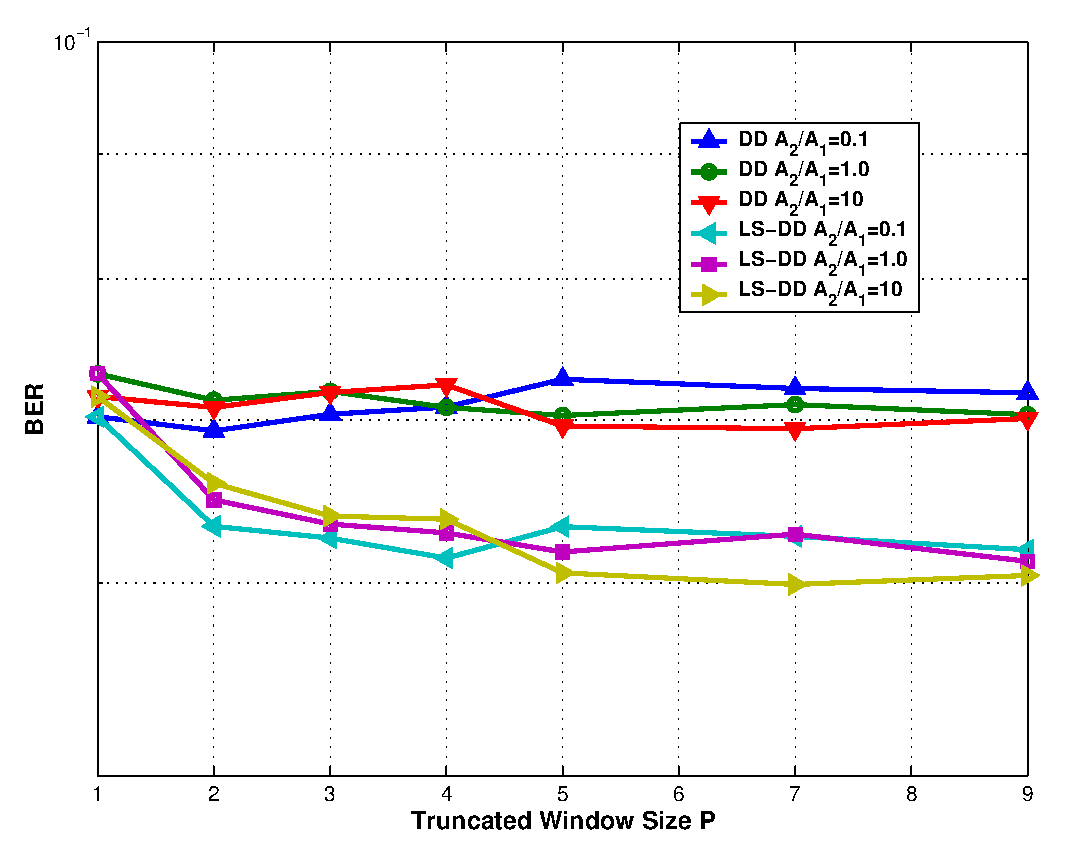
\includegraphics[width=4in]{P0.eps}}
\caption{Bit-error-rate comparison of the classic
signal-truncated-window decorrelating detector and the proposed LS
semi-blind detector against the window size $P$.} \label{P0}
\end{figure}

In figure \ref{P0}, the performance of the proposed LS semi-blind
detector is checked with the changing of the window size $P$. It
is easy to see that, when the single window is employed ($P=1$),
the performance of the proposed LS semi-blind detector is same to
that of the classic decorrelating detector. When multiple windows
are employed and $P>1$, the performance of the proposed LS
semi-blind detector is better than that of the classic
decorrelating detector. And the BER performance of the LS
semi-blind detector and the classic decorrelating detector is kept
unchanged against $A_2/A_1$.

\begin{figure}
\center{
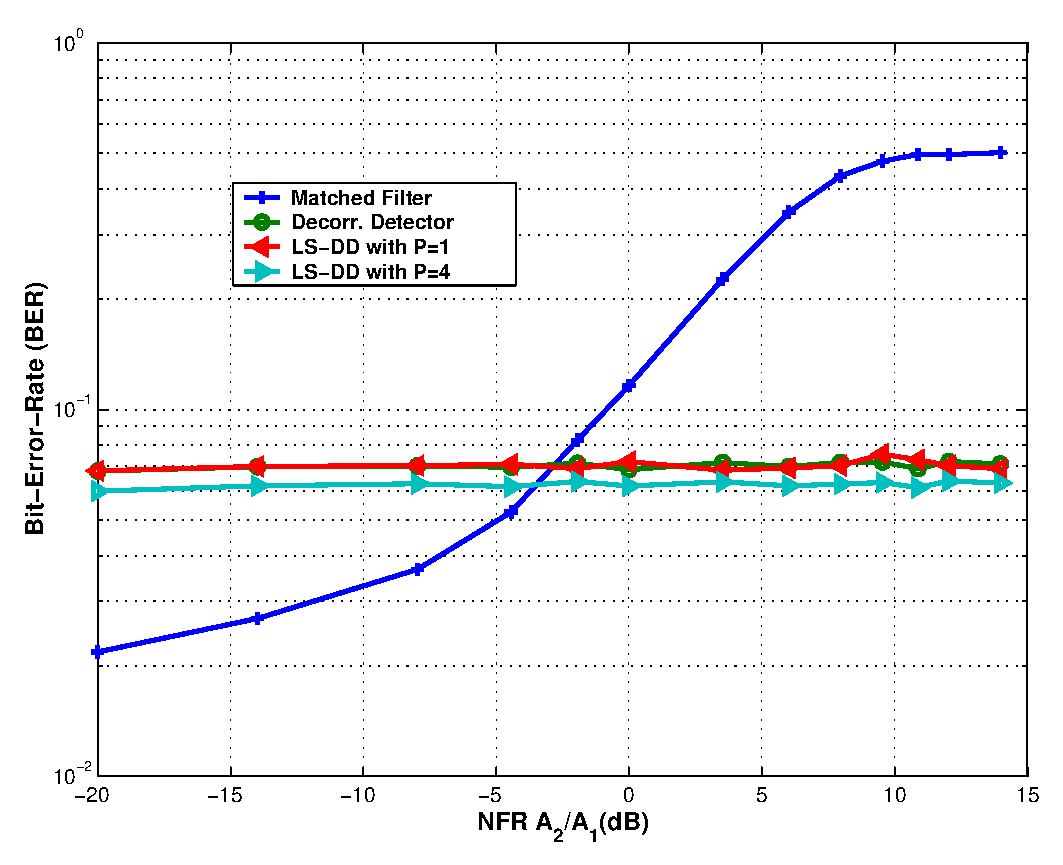
\includegraphics[width=4in]{NFR0.eps}}
\caption{NFR performance of the signal-user matched filter,
decorrelating detector, and the proposed LS semi-blind detector
with $P=1$ and $P=4$ for the first user within two users.}
\label{NFR0}
\end{figure}

Now, the NFR performance of the signal-user matched filter, the
classic single-truncated-window decorrelating detector and the
proposed LS semi-blind detector are checked in figure \ref{NFR0}.
As we see, the classic single-truncated-window decorrelating
detector and the proposed LS semi-blind detector have the same
optimum near-far resistance and their BERs are not change against
$A_2/A_1$. But the BER performance of the MF detector is
decreasing when $A_2/A_1$ becomes larger. Furthermore, the
performance of the proposed LS semi-blind detector with $P=4$ is
better than that of the classic single-window decorrelating
detector. And the proposed LS semi-blind detector with $P=1$ has
the similar performance to the classic single-window decorrelating
detector.

\subsection*{case 2: $\bar{\bN} \neq \mathbf{0}$}

In the case, we are dealing some more practical situations. So,
there would be the same level white Gaussian noise existing in the
blind signature matrix $\bcS$ as in the received signal vectors.
Then, both LS and MLS semi-blind detectors are used to detect the
expected signal.

\begin{figure}
\center{
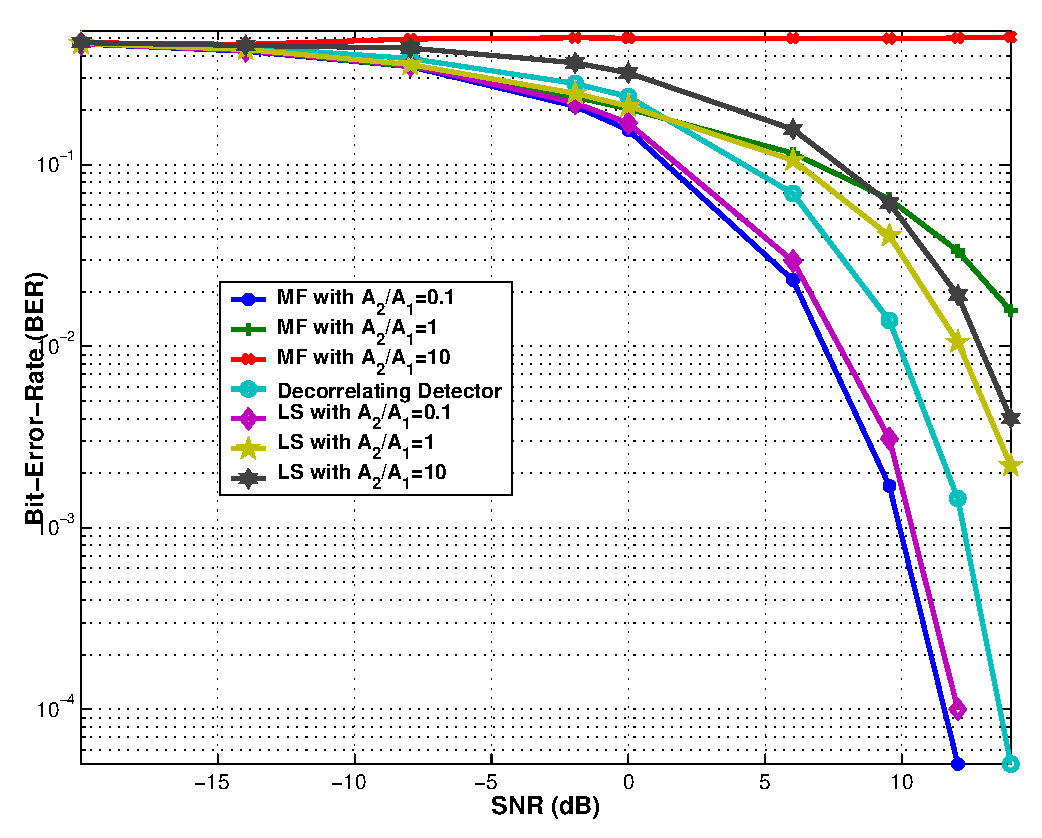
\includegraphics[width=4in]{BER_LS11.eps} }
\caption{Bit-error-rate comparison of the signal-user matched
filter, the single-truncated-window decorrelating detector, and
the proposed LS semi-blind detector with $P=1$ for the first user
within users.} \label{LS11}
\end{figure}

\begin{figure}
\center{
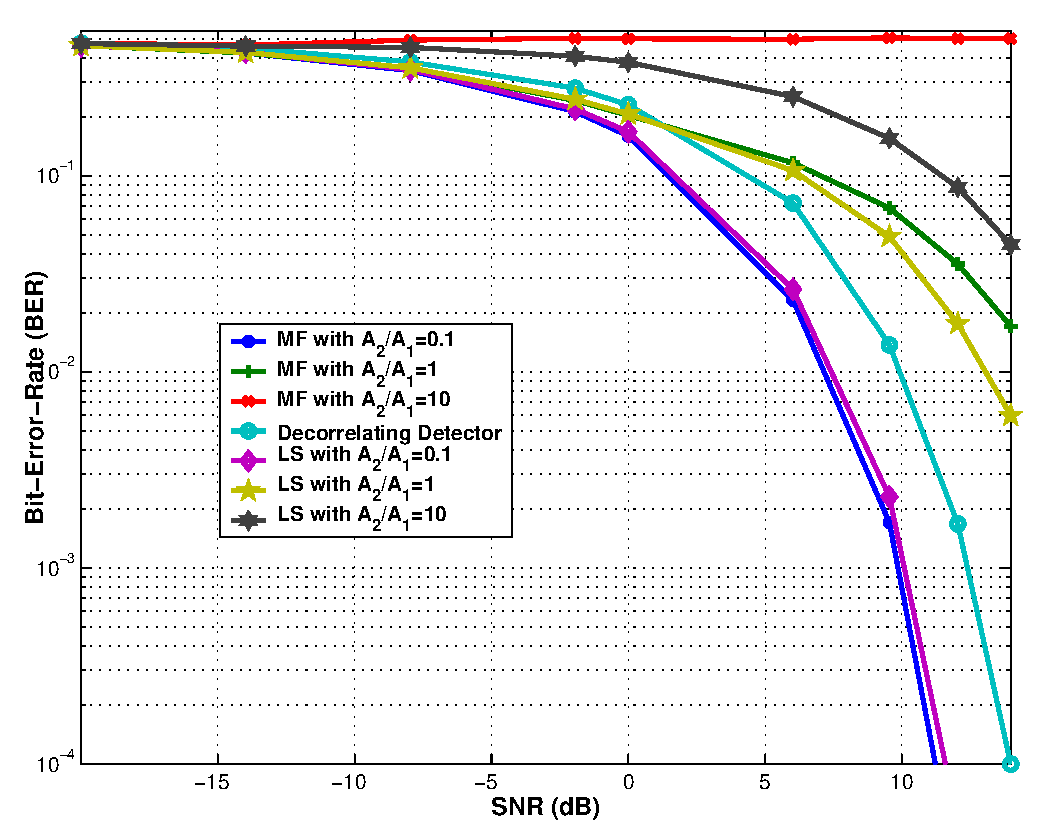
\includegraphics[width=4in]{BER_LS41.eps} }
\caption{Bit-error-rate comparison of the signal-user matched
filter, the single-truncated-window decorrelating detector, and
the proposed LS semi-blind detector with $P=4$ for the first user
within users.} \label{LS41}
\end{figure}

In figure \ref{LS11} and \ref{LS41}, the performance of the
proposed LS semi-blind detector with $P=1$ and $P=4$ is checked
against SNR and $A_2/A_1$, respectively. The most interesting is
that, when $A_2/A_1=0.1$, the performance of the proposed LS
semi-blind detector is very close to the MF detector and better
than that of the classic decorrelating detector. When $A_2/A_1=1$
or $10$, the performance of the LS semi-blind decorrelating
detector is decreased and is worse than that of the classic
decorrelating detector. But it is still better than that of the MF
detector. In this case, the performance of LS semi-blind detector
is always between those of the decorrelating detector and
single-user matched-filter detector.

On the other hand, when $A_2/A_1=0.1$, the performance of the
proposed LS semi-blind detector with $P=4$ is a little better than
that with $P=1$. But, when $A_2/A_1=10$, the performance of the
proposed LS semi-blind detector with $P=1$ is better than that
with $P=4$.

\begin{figure}
\center{
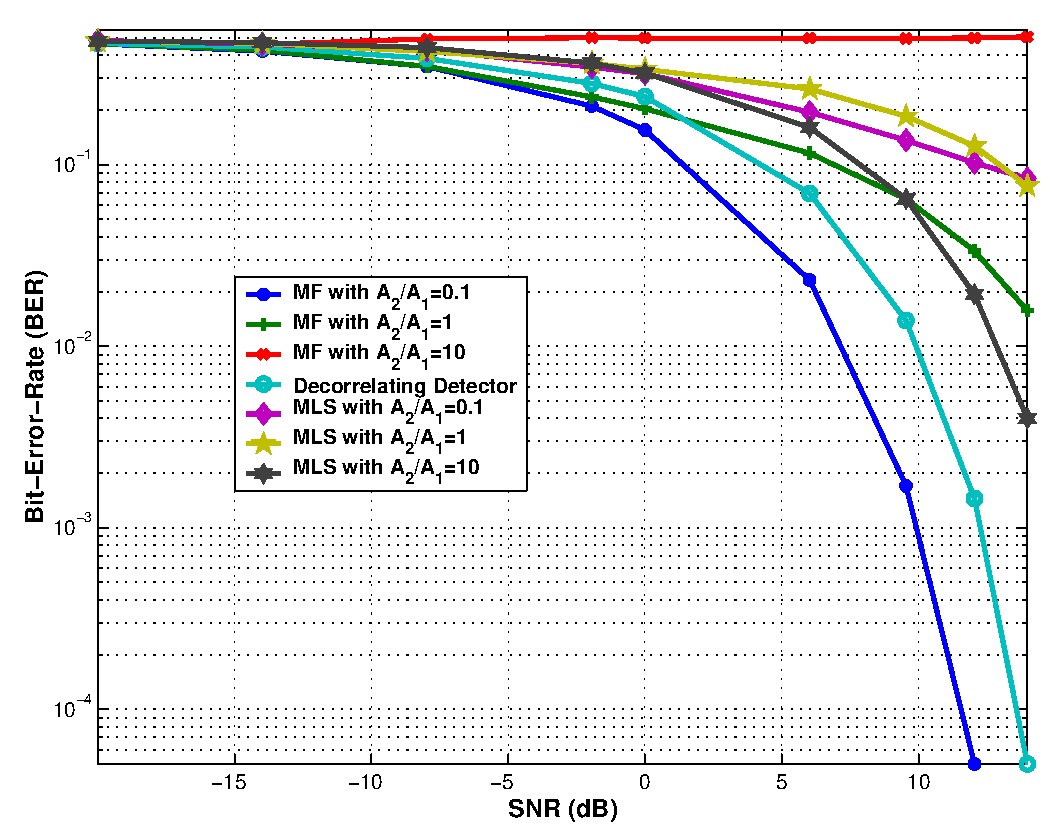
\includegraphics[width=4in]{BER_MLS11.eps}}
\caption{Bit-error-rate comparison of the signal-user matched
filter, the single-truncated-window decorrelating detector, and
the proposed MLS semi-blind detector with $P=1$ for the first user
within two users.} \label{MLS11}
\end{figure}


\begin{figure}
\center{
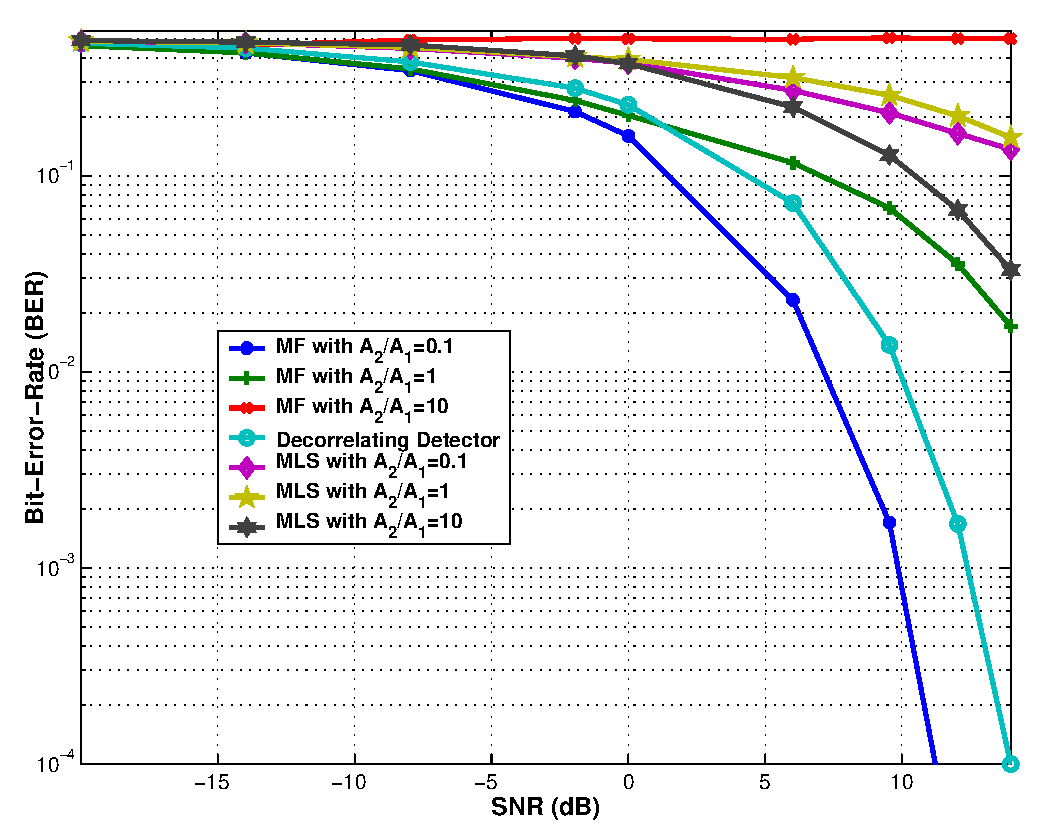
\includegraphics[width=4in]{BER_MLS41.eps}}
\caption{Bit-error-rate comparison of the signal-user matched
filter, the single-truncated-window decorrelating detector, and
the proposed MLS semi-blind detector with $P=4$ for the first user
within two users.} \label{MLS41}
\end{figure}

The BER performance of the proposed MLS semi-blind detector is
checked is checked in figure \ref{MLS11} and \ref{MLS41} against
SNR and $A_2/A_1$. As we see, the performance of the proposed MLS
detector is basically between that of the classic decorrelating
detector and MF detector when $A_2/A_1=10$.

\begin{figure}
\center{
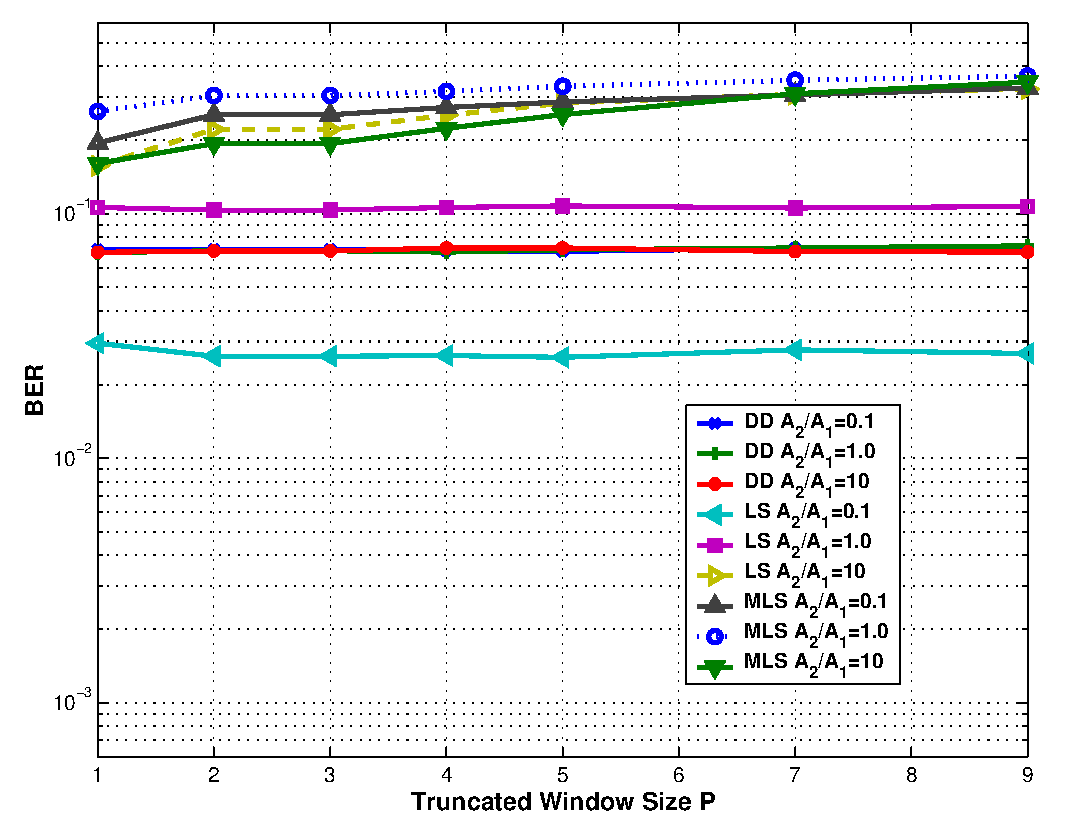
\includegraphics[width=4in]{P1.eps}}
\caption{Bit-error-rate comparison of the classic
signal-truncated-window decorrelating detector and the proposed LS
and MLS semi-blind detectors with against the window size $P$}
\label{P1}
\end{figure}

In figure \ref{P0}, we checked the performance of the proposed LS
and MLS multi-window semi-blind detector and the classic
single-truncated-window decorrelating detector, with the changing
of the window size $P$. As we see, except the performance of the
LS semi-blind detector with $A_2/A_1=0.1$ is better than that of
the classic decorrelating detector, the performance of the
proposed semi-blind detectors in the other case are not as good as
that of the classic decorrelating detector.

\begin{figure}
\center{
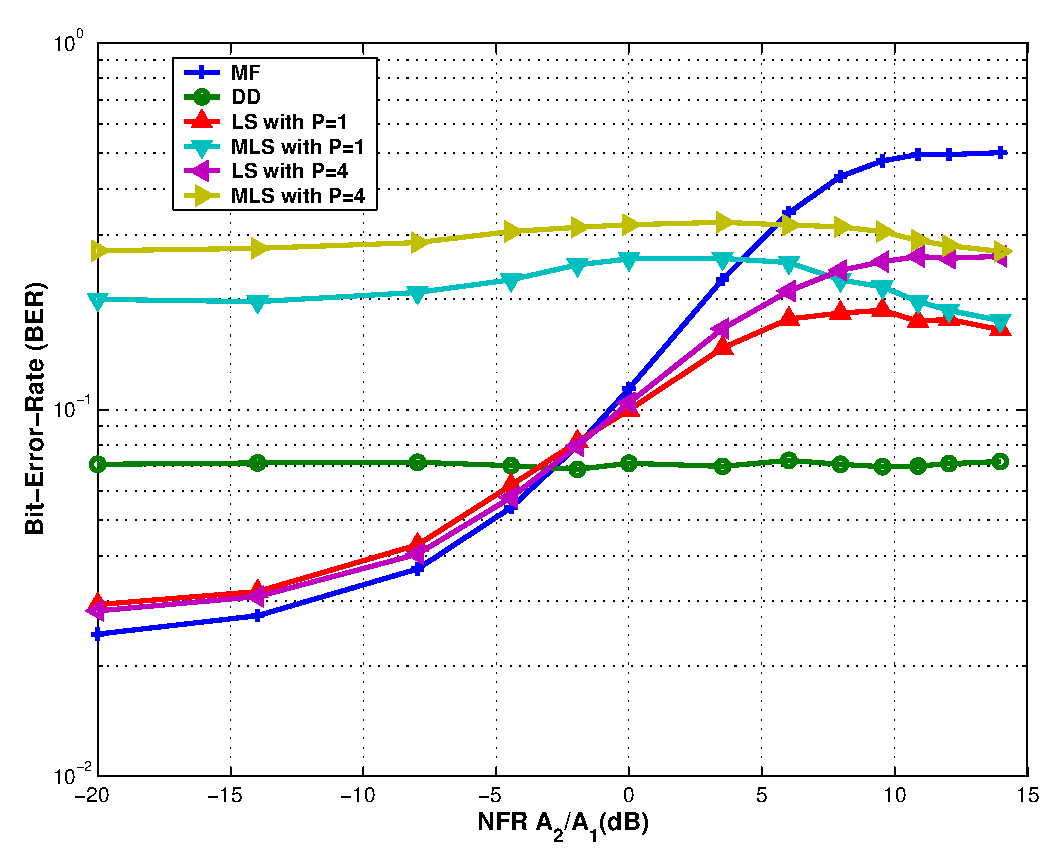
\includegraphics[width=4in]{NFR1.eps}}
\caption{Near-far resistance comparison of the signal-user matched
filter, single-truncated-window decorrelating detector, and the
proposed LS and MLS semi-blind detectors for the first user within
two users. $SNR=6dB$} \label{NFR1}
\end{figure}

In figure \ref{NFR1}, we check the NFR performance of the
signal-user matched filter, the classic single-truncated-window
decorrelating detector, and the proposed LS  and MLS semi-blind
detector with $P=1$ and $P=4$. Firstly, the BER performance of the
proposed MLS semi-blind detector with $P=1$ or $P=4$ is basically
not changed against $A_2/A_1$. From figure \ref{LS11} and
\ref{LS41}, we can see that the performance of the LS semi-blind
detector is between that of the MF detector and the classic
decorrelating detector. When $A_2/A_1$ is large enough, the
performance of the LS semi-blind detector with $P=1$ and $P=4$ is
closed to that of the MLS semi-blind detector with $P=1$ and
$P=4$, respectively.

\section{Conclusions}

In this paper, we presented the one-shot LS and MLS semi-blind
decorrelating detectors with the multiple consecutive truncated
windows. In these two semi-blind multi-windows decorrelating
detector, besides the signature and timing of the desired user,
the amplitude of this user is also required. This is why they are
called semi-blind detectors. In the theoretical analysis and
computer simulations, as we may see, when there is no noise in the
semi-blind signature matrix $\bcS$ and $P=1$, the classic
single-truncated-window decorrelating detector is just one special
case of the presented LS semi-blind detector with $\bB=\bI$. And
when there is no noise in the semi-blind signature matrix, the
performance of the LS semi-blind detector with multiple windows is
better than that with $P=1$ and the classic
single-truncated-window decorrelating detector.

These two semi-blind decorrelating detectors are simple and
direct. No searching or converging procedure is required as in
other semi-blind/semi-blind detectors.

\bibliographystyle{unsrt}
\bibliography{J-AsynchSemiBlindDetector10}
\end{document}
